\section{Antenner för kortvåg}

\subsection{Mittmatad halvvågsantenn}
\textbf{
HAREC a.\ref{HAREC.a.6.1.1}\label{myHAREC.a.6.1.1}
}

Se föregående avsnitt

\subsection{Ändmatad halvvågsantenn}
\textbf{
HAREC a.\ref{HAREC.a.6.1.2}\label{myHAREC.a.6.1.2}
}

Utstrålningen från en halvvågsantenn är i princip lika hur den än
matas. En ändmatad halvvågsantenn fungerar m.a.p. strålningsriktningar
på samma sätt som en mittmatad. Vid längre antenner blir
strålningskaraktären däremot en annan.

Skillnaden mellan änd- och mittmatade halvvågsdipoler är att
anslutningsimpedansen är mycket högre i ändarna än i mitten. För att
mata antennen längst ut i ena änden behövs en transmissionsledning med
hög impedans, varvid ledningens ena part ansluts till antennen och den
andra parten lämnas fri. En sådan anordning kallas zeppantenn och
användes först i luftskepp, s.k. zeppelinare.

\hilight{TODO:  Här borde vi ta upp att Zepp-antennen och J-pole är olika namn
på samma sak, samt förklara att J-pole, trots vad ''folk på nätet skriver'',
kräver balun och att den inte kan jordas.}

\subsection{Omvikt dipol (folded dipole)}
\textbf{
HAREC a.\ref{HAREC.a.6.1.3}\label{myHAREC.a.6.1.3}
}

\begin{wrapfigure}{R}{0.5\textwidth}
  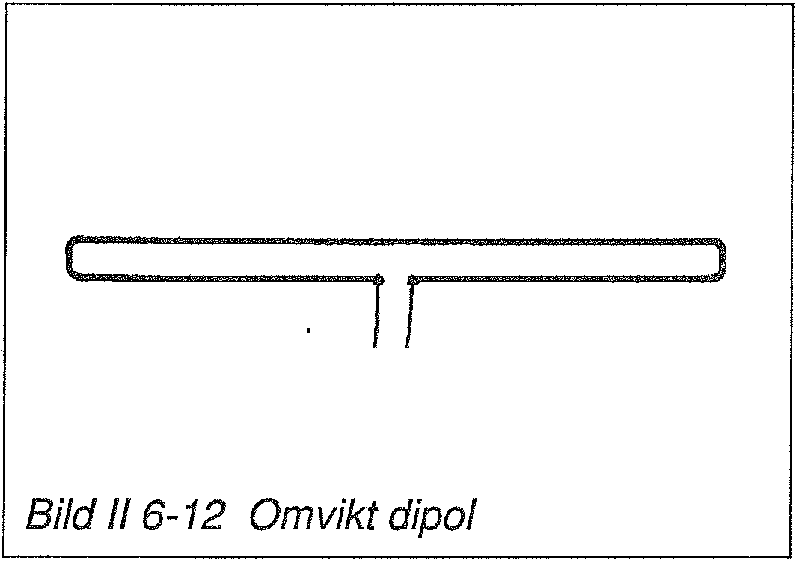
\includegraphics[width=0.5\textwidth]{images/bild_2_6-12}
  \caption{Omvikt dipol}
  \label{fig:bildII6-12}
\end{wrapfigure}

Bild \ref{fig:bildII6-12}

En omvikt dipol kan ses som två eller flera parallella element, som är
sammankopplade i ändarna. Mittpunkten på ett av elementen är ansluten
till antennledningen.

Matningsimpedansen för en omvikt \(\lambda/2\)-dipol med två element är
ca fyra gånger högre än den för en enkel dipol, d.v.s. 200--300~Ω.
Den omvikta dipolen, som endast fungerar på grundfrekvensen och på
dess udda övertoner, är relativt bredbandig. Matningsimpedansen kan
ändras med sinsemellan olika diametrar på de ingående elementen samt
med antalet parallellkopplade element.

\subsection{Jordplanantenn}
\textbf{
HAREC a.\ref{HAREC.a.6.1.4}\label{myHAREC.a.6.1.4}
}

\begin{wrapfigure}{R}{0.5\textwidth}
  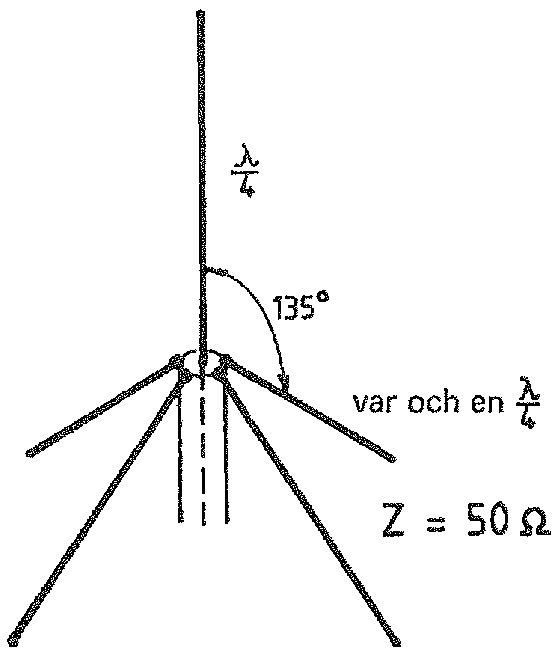
\includegraphics[width=0.5\textwidth]{images/bild_2_6-13}
  \caption{GP-antenn}
  \label{fig:bildII6-13}
\end{wrapfigure}

Bild \ref{fig:bildII6-13}

Jordplanantennen eller GP-antennen (GP av ground plane) består av en
lodrät strålare som den ena polen och flera sammankopplade
\(\lambda/4\)-radialer eller markplanet som den andra polen.

GP-antennen är rundstrålande och har vertikal polarisering. Dess
relativt flacka utstrålning, i jämförelse med en horisontell antenn,
gör den lämpad för långa distanser. Av mekaniska skäl används den
mest på högre frekvenser (14~MHz och högre).

Med horisontella radialer som jordplan är matningsimpedansen ca 35~Ω.
För att få god impedansanpassning, t.ex. till en 50~Ω koaxialkabel
som matarledning, görs radialerna sluttande nedåt i en lämplig vinkel.

Koaxialkabelns innerledare ansluts till antennen och kabelskärmen till
radialerna.

Om antennen placeras omedelbart ovan markytan, kan marken användas som
jordplan, särskilt om dess elektriska ledningsförmåga är god.

Bild \ref{fig:bildII6-14}

Om antennelementet inte har en elektrisk längd av \(\lambda/4\), kan
längden anpassas elektriskt på liknande sätt som beskrivits tidigare i
detta kapitel för dipolantenner.

\begin{figure}
  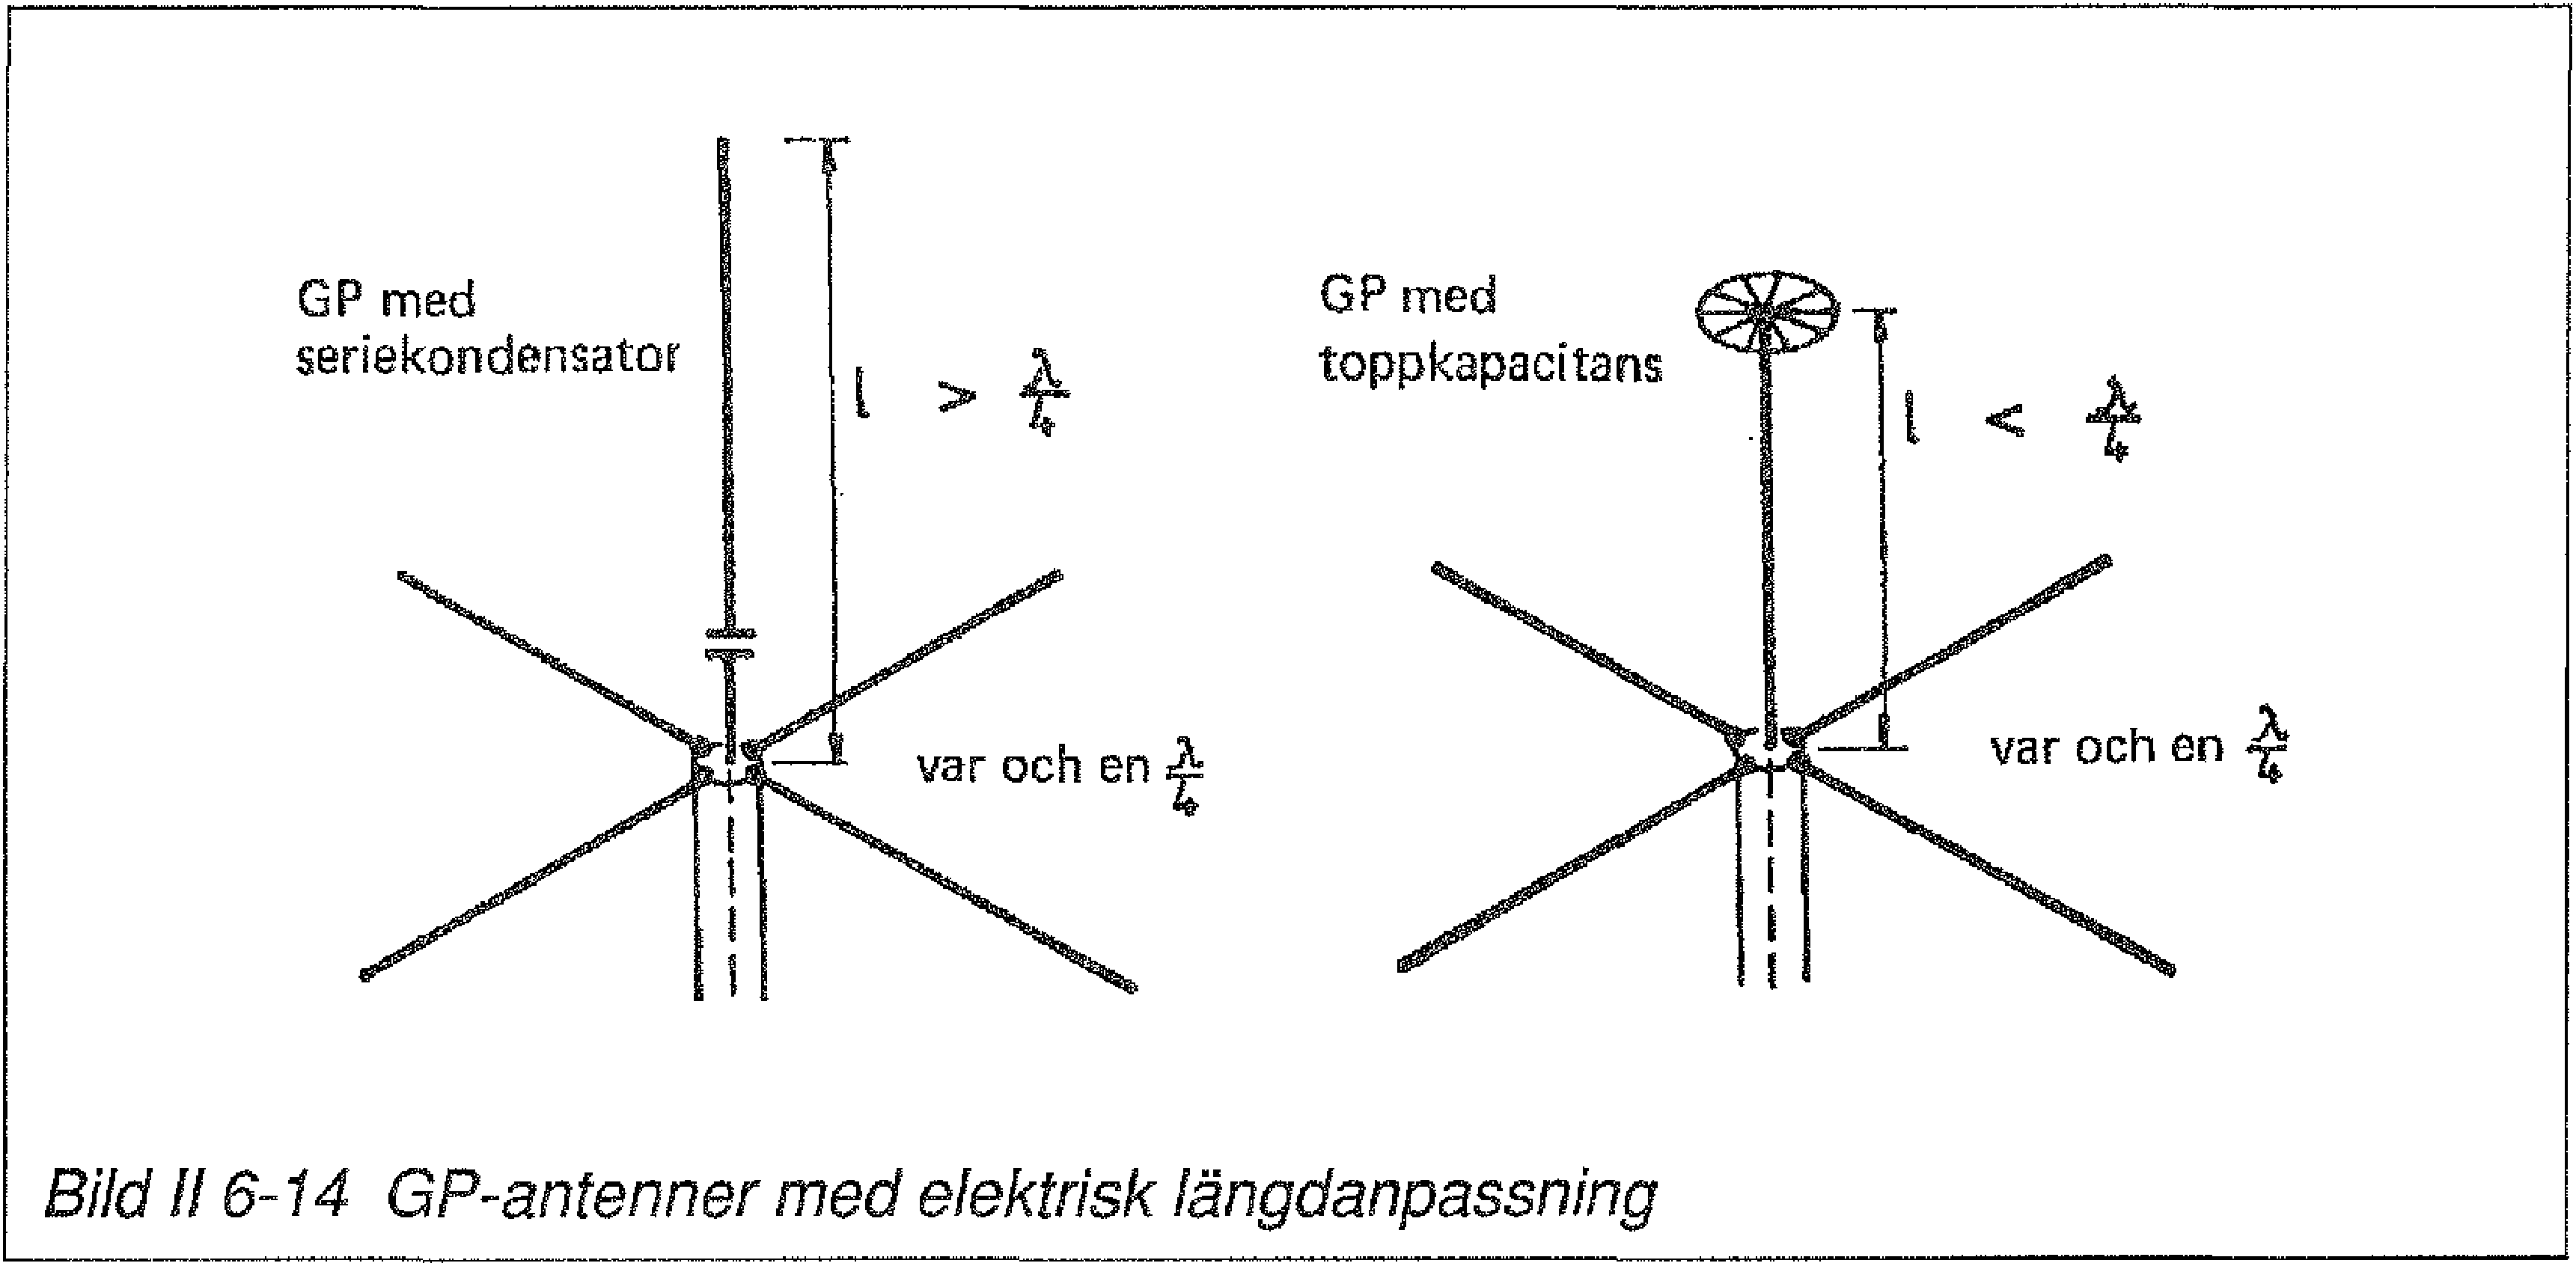
\includegraphics[width=\textwidth]{images/bild_2_6-14}
  \caption{GP-antenner med elektrisk längdanpassning}
  \label{fig:bildII6-14}
\end{figure}

\subsection{Flerbands GP-antenner}

En GP-antenn kan fås att fungera på flera band genom inbyggnad av en
spärrkrets i antennelementet för tillkommande band och av
jordplansradialer med anpassad längd eller med spärrkretsar även i
jordplanet för de banden.

Antennen fungerar som \(\lambda/4\) GP-antenn åtminstone på de lägsta
banden. Den mekaniska längden på en flerbands GP för kortvåg blir
kort, 4 à 6,5~meter, vilket på de lägre banden innebär dålig
verkningsgrad och liten bandbredd. Jämför med SVF-kurvorna på
bilden. Flerbands GP-antenner för upp till sju kortvågsband
tillverkas.

Bild \ref{fig:bildII6-15}

\begin{figure}
  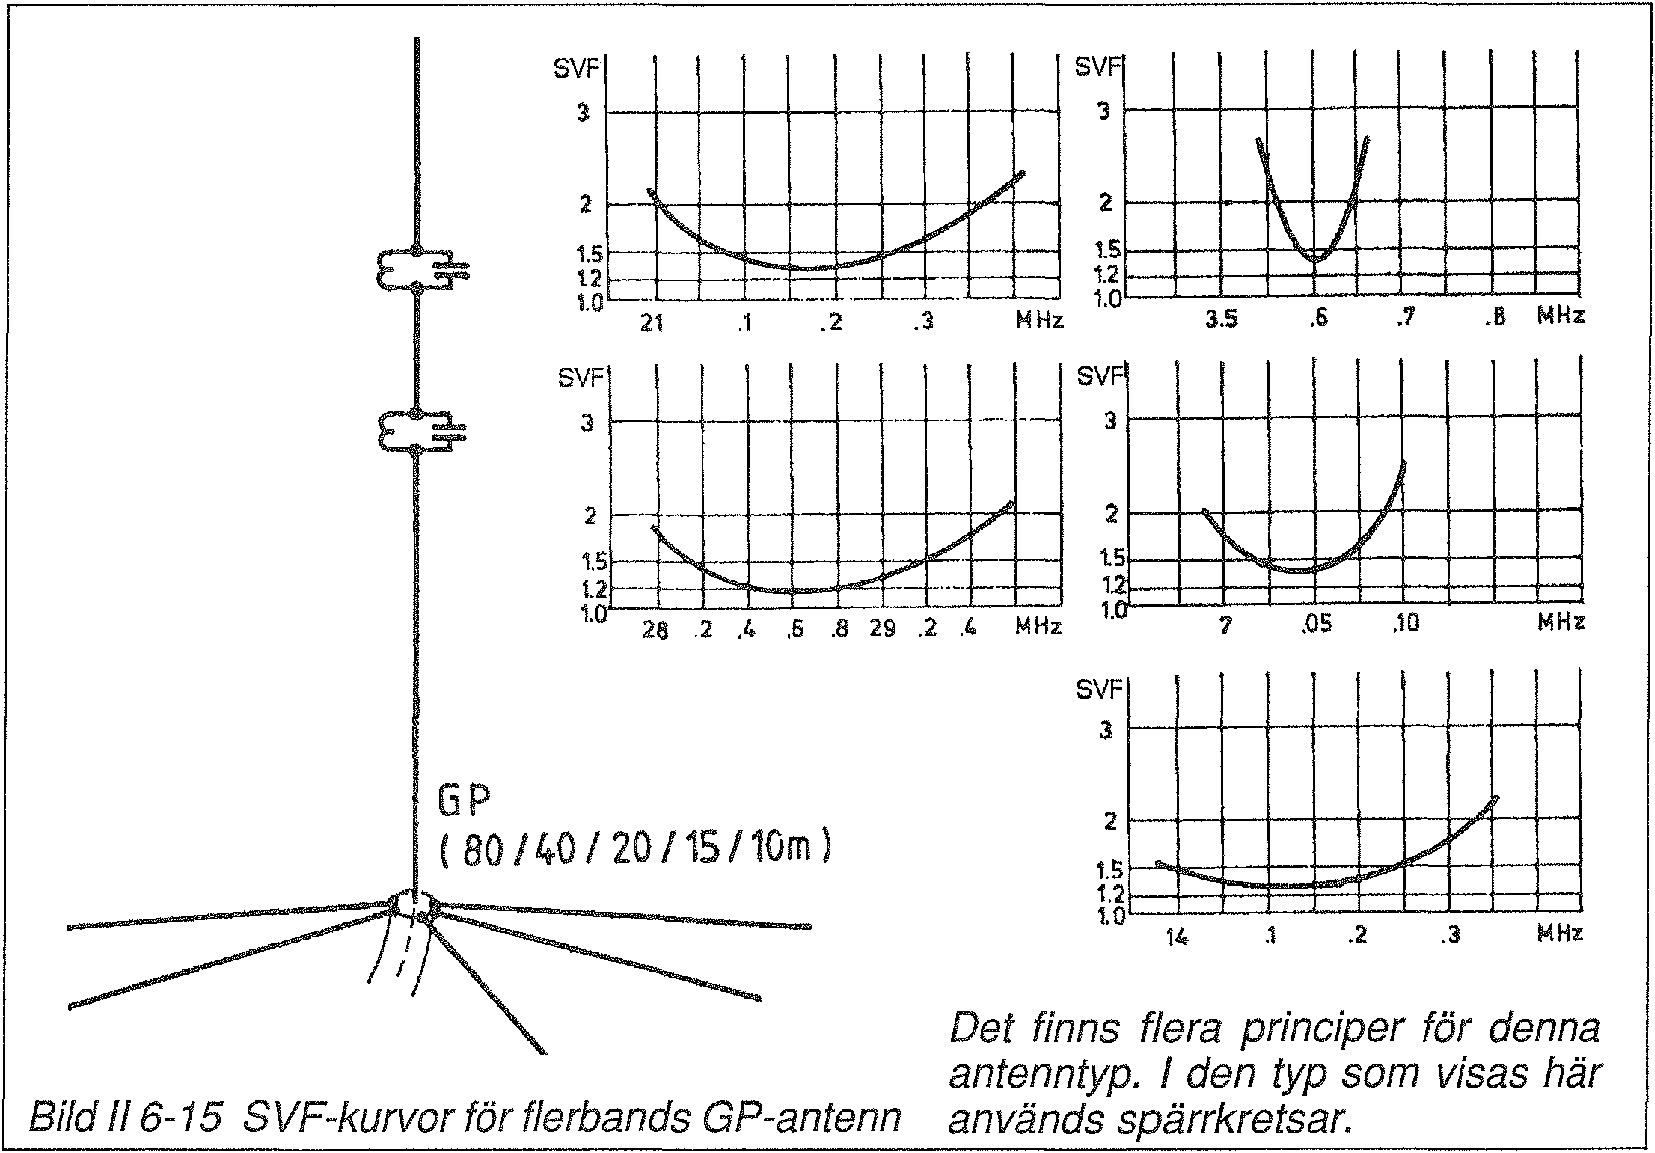
\includegraphics[width=\textwidth]{images/bild_2_6-15}
  \caption{SVF-kurvor för flerbands GP-antenn}
  \label{fig:bildII6-15}
\end{figure}

\subsection{Flerbands halvvågsantenner}
\textbf{
HAREC a.\ref{HAREC.a.6.1.7}\label{myHAREC.a.6.1.7}
}

Bild \ref{fig:bildII6-16}
\label{W3DZZ}

En vanligt förekommande flerbandsantenn är W3DZZ-antennen (namnet
efter konstruktörens anropssignal). Den är en oftast horisontellt
upphängd dipolantenn för 80, 40, 20, 15 och 10~m-banden.

W3DZZ-antennen är ca 33,6~meter lång och har två spärrkretsar,
symmetriskt utplacerade omkring matningspunkten. Matningen sker med
koaxialkabel och balun.

Antennen har en matningsimpedans av ca 50~Ω på 80- och
40-metersbanden På de högre banden är anpassningen inte optimal --
matningsimpedansen stiger där upp till ca 120~Ω. Många använder
bl.a. av den anledningen inte W3DZZ-antennen på höga kortvågsband utan
föredrar där en flerbandig GP-antenn eller en riktantenn (Yagi, quad
m.fl.).

\begin{figure}
  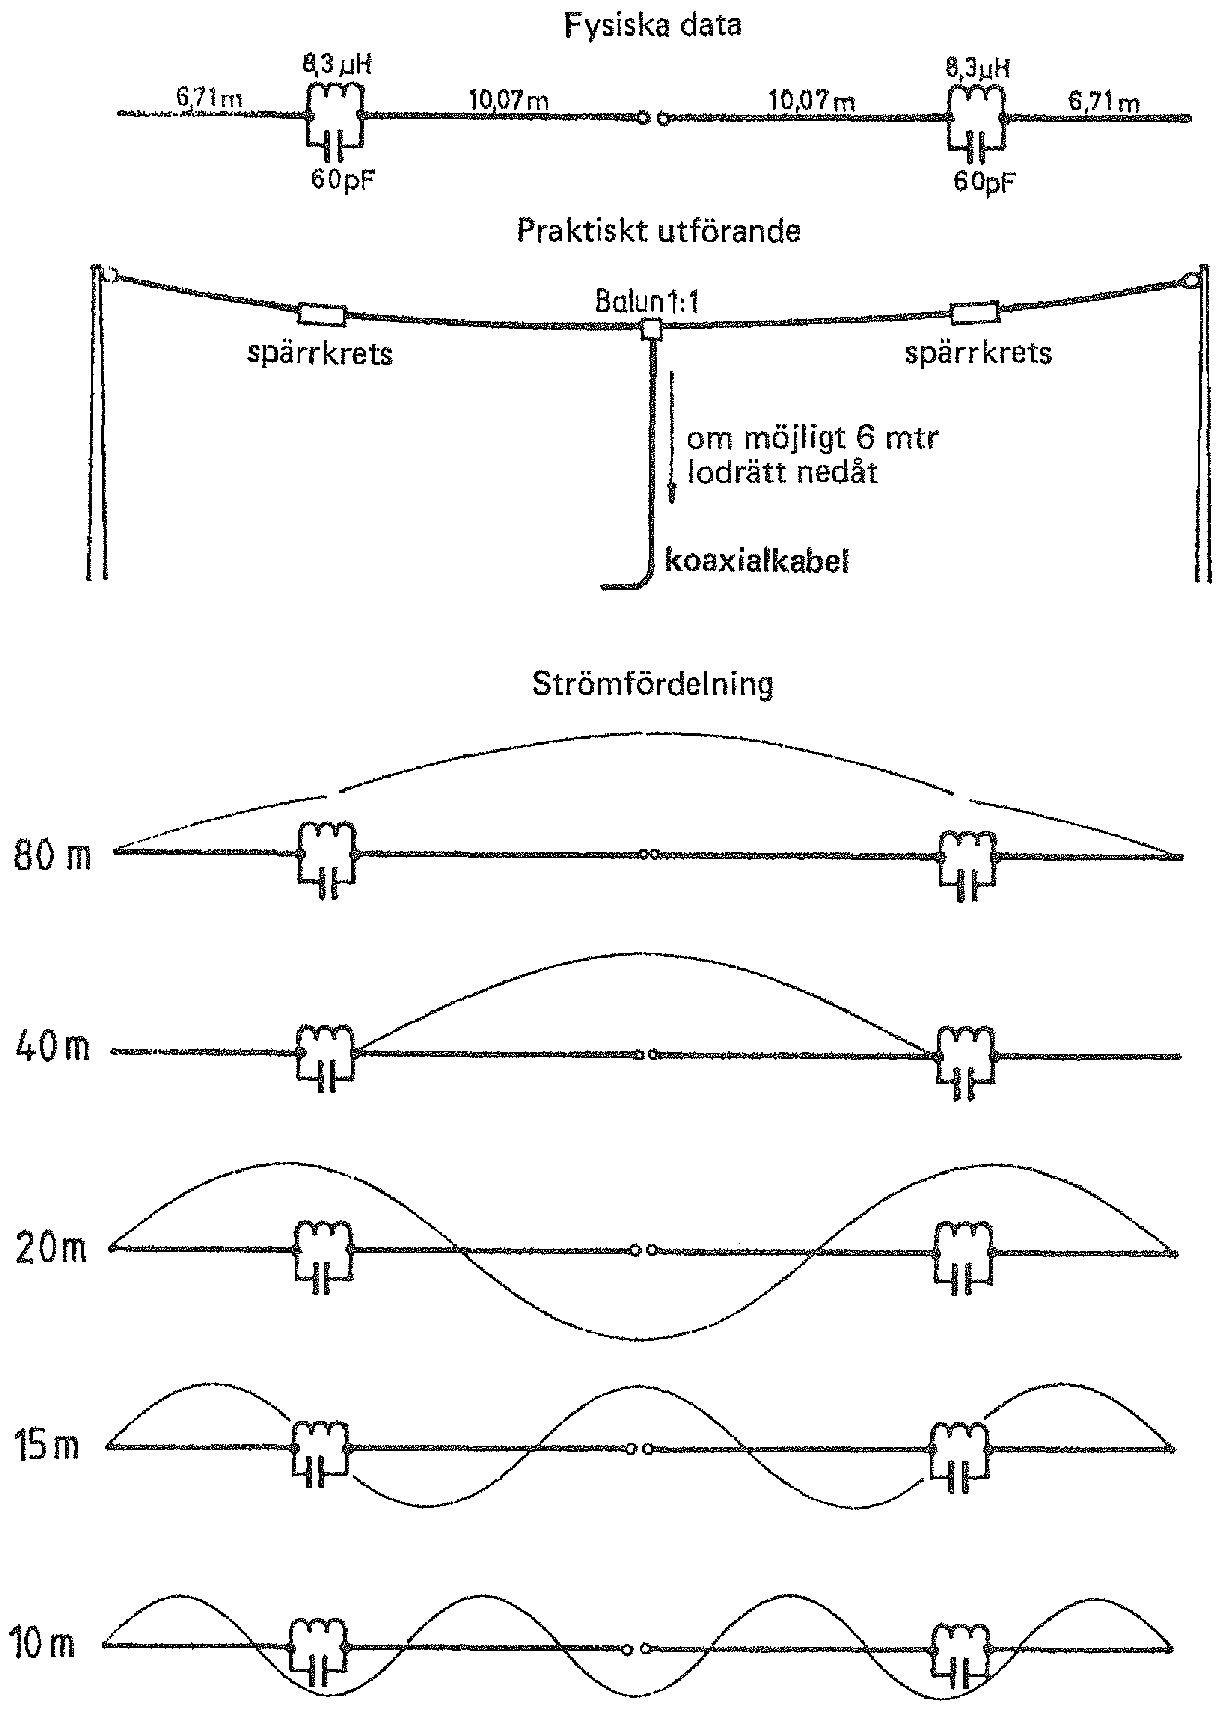
\includegraphics[width=\textwidth]{images/bild_2_6-16}
  \caption{W3DZZ-antennen}
  \label{fig:bildII6-16}
\end{figure}

W3DZZ-antennens arbetssätt:
\begin{itemize}
  \item 80 m-bandet \\ Hela antennen fungerar som en
    \(\lambda/2\)-dipol med resonansfrekvensen 3,7~MHz. Den mekaniska
    längden är \(2 \cdot 16,8\) meter och förlängs elektriskt med
    induktanserna i spärrkretsarna, vilka f.ö. är ur resonans på detta
    band.
  \item 40 m-bandet \\ Spärrkretsarna är i resonans och ''kopplar
    bort'' antenndelen utanför dem. Delen där innanför fungerar som en
    \(\lambda/2\)-dipol med resonansfrekvensen 7,05~MHz.

  \item 20 m-bandet \\ Hela antennen fungerar som \(3\lambda/2\)-dipol
    med resonansfrekvensen 14,1~MHz.

  \item 15 m-bandet \\ Hela antennen fungerar som \(5\lambda/2\)-dipol
    med resonansfrekvensen 21,2~MHz.

  \item 10 m-bandet \\ Hela antennen fungerar som \(7\lambda/2\)-dipol
    med resonansfrekvensen 28,4~MHz.
\end{itemize}
